O método proposto neste trabalho é apoiado por um ambiente computacional formado por três componentes: módulo de colaboração, módulo de processamento, e módulo de apresentação. O fluxo de dados entre os componentes pode ser observado na Figura~\ref{fig:ambiente}.

\begin{figure}[ht]
\centering
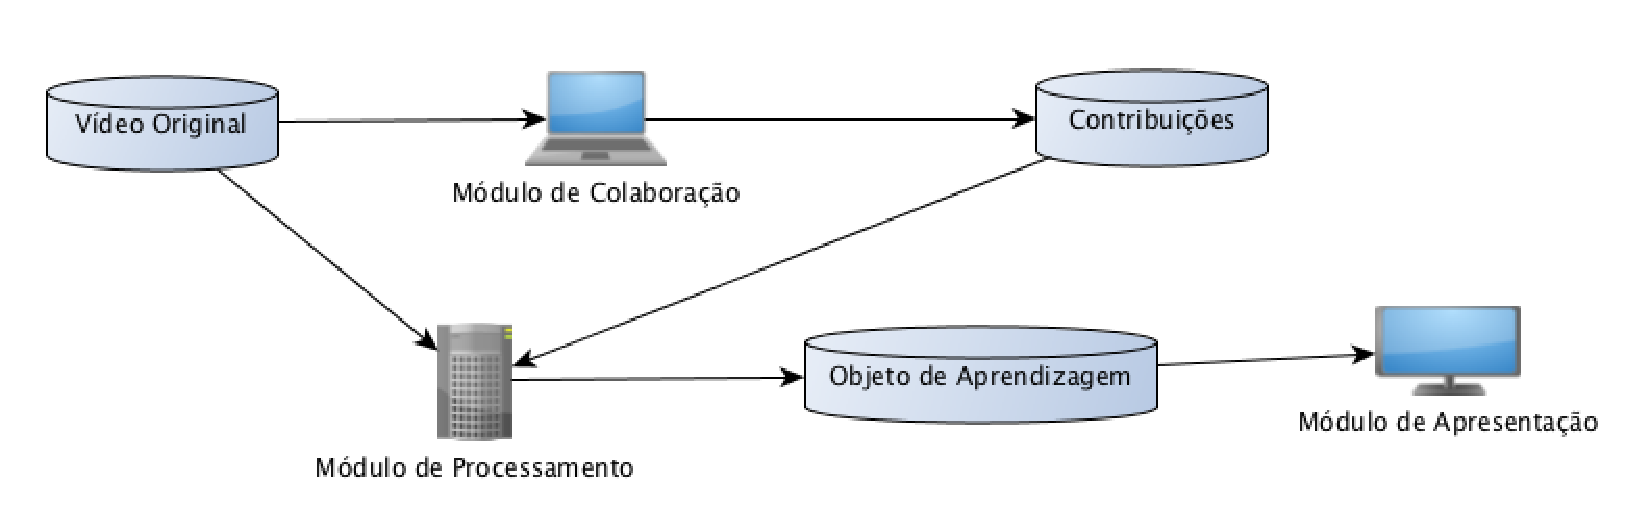
\includegraphics[width=.99\textwidth]{imagens/ambiente.eps}
\caption{Componentes do Ambiente de Apoio}
\label{fig:ambiente}
\end{figure}

O módulo de colaboração apoia as atividades de obtenção das informações necessárias para gerar o conteúdo complementar, a ser utilizado para enriquecer os vídeos. Por meio das ferramentas contidas nesse módulo, os estudantes podem contribuir de três maneiras: identificando lacunas semânticas, sugerindo conteúdos complementares para cobri-las, ou validando contribuições de outros estudantes. Esse módulo se baseia em uma abordagem crowdsourcing, que oferece suporte aos cenários de colaboração em escala massiva, além de propor formas eficientes de divisão e distribuição de tarefas, assim como de validação e agregação das contribuições. 

O módulo de processamento utiliza técnicas baseadas em modelos e funções paramétricas para gerar, a partir das contribuições dos estudantes, o conteúdo multimídia a ser agregado aos vídeos. Para este projeto foram selecionados três tipos de conteúdo: hiperlinks, caixas de texto e imagens. Os hiperlinks são inseridos em pontos do vídeo que requerem informação adicional, e apontam para outros vídeos ou páginas web com mais informações sobre os respectivos conceitos. As caixas de texto são utilizadas para contextualizar fatos e informações, para adicionar informações complementares, e para listar formas equivalentes para termos e expressões. As imagens são utilizadas para ajudar a explicar conceitos, apresentando desenhos, gráficos e fotografias que ajudem o estudante a compreender o conteúdo apresentado. 

O módulo de apresentação é utilizado para exibir os objetos de aprendizagem, com todas as funcionalidades necessárias para que o estudante possa interagir com eles. Adicionalmente esse módulo oferece funcionalidades que permitem aos estudantes fazerem recomendações, avaliações e sugestões de modificações nos objetos de aprendizagem.